% fork-existence.tex

\documentclass[border={10pt 10pt 10pt 10pt}]{standalone}

\usepackage{tikz}
\usetikzlibrary{shapes, positioning, arrows.meta, decorations.pathmorphing}

\begin{document}
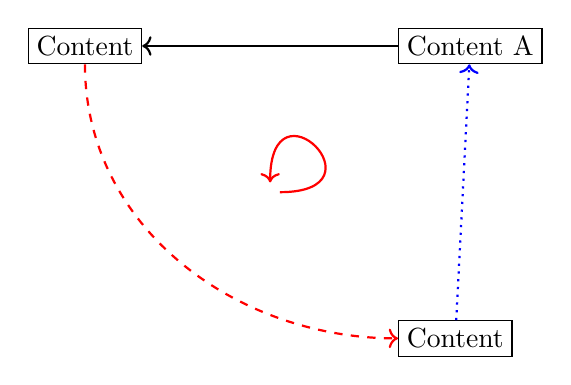
\begin{tikzpicture}[
    node distance = 1.5cm and 1.5cm,
    sa/.style = {->, thick},
    sb/.style = {->, thick, dashed, red},
    sc/.style = {->, thick, dotted, blue},
    n/.style = {draw, inner sep = 3pt, align = center}]

  \node[] (l) {};
  \node[n, above right = of l] (ta)
  {Content A};
  \node[n, above left = of l] (tb)
  {Content};
  \node[n, below right = of l] (tc)
  {Content};
  \draw[sa, sloped] (ta) to (tb);
  \draw[sb] (tb) to[out=-90,in=180] (tc);
  \draw[sc, sloped] (tc) to (ta);
  \draw[->,red,thick] (l) to[out=0, in=90, looseness=20] (l);
\end{tikzpicture}
\end{document}